\documentclass[11pt]{article}
\usepackage[margin=1in]{geometry}
\usepackage{amsmath,amssymb,amsthm,mathtools}
\usepackage{microtype,graphicx,booktabs}
\usepackage{algorithm,algpseudocode,xurl}
\usepackage[colorlinks=true,linkcolor=blue,citecolor=blue,urlcolor=blue]{hyperref}
\hypersetup{pdftitle={Local approximation widths for elliptic equations with measurable coefficients},
 pdfauthor={Kaiwen Jin},pdfsubject={AIM Problem 517}}
\newtheorem{theorem}{Theorem}[section]
\newtheorem{lemma}[theorem]{Lemma}
\theoremstyle{remark}
\newtheorem{remark}[theorem]{Remark}
\newcommand{\R}{\mathbb R}
\newcommand{\Ha}{\mathcal H_A}
\newcommand{\norma}[2]{\|#1\|_{a,#2}}
\newcommand{\Tr}{\operatorname{tr}}
\newcommand{\dd}{\,\mathrm d}
\newcommand{\mean}[2]{\frac{1}{|#2|}\int_{#2}#1}
\DeclareMathOperator{\dist}{dist}
\title{Local approximation widths for elliptic equations\protect\\ with measurable coefficients}
\author{Kaiwen Jin\\\small\href{mailto:yui.ui.siki@gmail.com}{\texttt{yui.ui.siki@gmail.com}}}
\date{11 October 2026}
\begin{document}
\maketitle
\begin{abstract}
We prove that the local energy approximation widths of scalar, symmetric,
uniformly elliptic equations in dimensions two and three decay as
$\exp(-c n^{1/(d-1)})$, with no regularity assumption on the coefficients
beyond measurability and boundedness. The result applies to the normalized
cutoff operator on nested cubes in AIM Problem 517. Its proof compares
the derivative of a harmonic energy Gram matrix with tangential boundary
energy, and the Gram matrix itself with the energy of an ordinary harmonic
extension. Spherical harmonic counting then bounds the determinant and
the restriction singular values. A finite ball covering transfers the
estimate to the prescribed cutoff. Exact propagation through radial
layers supplies reproducible numerical checks of the determinant estimate.
The constants may depend on coefficient contrast.
\end{abstract}

\section{Introduction and main result}
Local spaces of solutions of an elliptic equation provide coefficient-adapted
basis functions for multiscale approximation. Their Kolmogorov widths measure
the best error attainable with a prescribed local dimension, after allowing
solutions on a larger domain. The cutoff formulation used in generalized
finite element methods retains the partition of unity in the approximation
norm; see Ma, Scheichl and Dodwell \cite[Section 3.1]{MSD2021}.
For the scalar elliptic case, Ma's abstract theory gives decay with exponent
$1/d$ \cite[Theorem 3.8, Remark 3.9 and Section 6.1]{Ma2024};
Section 7 of that preprint asks for the exponent $1/(d-1)$.

For ordinary harmonic functions, the boundary dimension already determines
singular-value decay. In their author-hosted final text, Bandtlow and Chu
give exact ball formulas in the
$L^2$ harmonic Bergman setting and extend the decay to relatively compact
domain pairs by ball covers \cite[Proposition 3.3 and Theorem 4.5]{BandtlowChu2009}.
Measurable elliptic coefficients do not preserve that explicit harmonic
expansion. We instead compare two quadratic forms on almost every sphere;
the reference spherical harmonics enter only in a variational estimate.
This yields the same exponent for the energy restriction and for the
scalar cutoff widths asked for in AIM Problem 517 \cite{AIM517}.

Let $d\in\{2,3\}$ and let
$\omega\Subset\omega^*\subset\R^d$ be concentric open cubes. Suppose
$A\in L^\infty(\omega^*;\R^{d\times d})$ is real symmetric and
\begin{equation}\label{eq:ellipticity}
 \alpha |\xi|^2\le \xi^T A(x)\xi\le\beta|\xi|^2,
 \qquad 0<\alpha\le\beta<\infty,
\end{equation}
for almost every $x$ and every $\xi\in\R^d$. For a subdomain $D$ set
\[
 a_D(u,v)=\int_D A\nabla u\cdot\nabla v\dd x,\qquad
 \norma{u}{D}=a_D(u,u)^{1/2}.
\]
This is a seminorm until constants have been removed. Fix a nonzero
$\chi\in W^{1,\infty}(\omega)\cap H^1_0(\omega)$ and define
\begin{align*}
 \Ha(\omega^*)&=\{u\in H^1(\omega^*):
 a_{\omega^*}(u,v)=0\text{ for every }v\in H^1_0(\omega^*)\},\\
 \Ha^0(\omega^*)&=\{u\in\Ha(\omega^*):a_\omega(\chi u,\chi)=0\}.
\end{align*}
For $Tu=\chi(u|_\omega)$, the width in the target energy norm is
\begin{equation}\label{eq:width}
 d_n(T)=\inf_{\substack{V\subset H^1_0(\omega)\text{ linear}\\\dim V\le n}}
 \ \sup_{\substack{u\in\Ha^0(\omega^*)\\\norma{u}{\omega^*}\le1}}
 \ \inf_{v\in V}\norma{Tu-v}{\omega}.
\end{equation}

\begin{theorem}\label{thm:main}
For every fixed choice of the preceding data, there are $C,c>0$, independent
of $n$, such that
\[
 d_n(T)\le C\exp\bigl(-c n^{1/(d-1)}\bigr)
 \qquad\text{for every integer }n\ge1.
\]
\end{theorem}
The spaces, normalization and norms in \eqref{eq:width} are identical to
those in Problem 517, so Theorem~\ref{thm:main} proves its proposed bound
for every admissible coefficient and cutoff. No smoothness or scale separation
of $A$ is imposed. We do not claim contrast-independent constants or a
matching lower bound for every cutoff. The exact ordinary harmonic ball
model has this exponent, as described in Section~\ref{sec:numerics}.

The proof estimates the growth of the determinant of an energy Gram matrix
on expanding balls. Boundary spectral estimates and energy determinants
also appear in Li and Wang's dimension bounds for harmonic functions
\cite[Lemma 1 and Section 2]{LiWang2000}; we use a local comparison with
the ordinary harmonic extension. The key inequalities are an upper bound
for the interior energy by that extension energy, and a lower bound for
its radial derivative by tangential boundary energy. Their combination
avoids differentiating the coefficient. Almost-everywhere Sobolev slicing
and a separate singular-Gram-matrix case make the argument applicable at
the stated regularity. Section~\ref{sec:balls} proves the ball estimate,
Section~\ref{sec:cubes} transfers it to the cutoff, and
Section~\ref{sec:numerics} describes radial computations. All spaces are
real, and surface integrals use ordinary area measure.

\section{Energy restriction on balls}\label{sec:balls}
Write $B_t=B_t(0)$; translation gives balls with any center.
Throughout this section $A$ satisfies \eqref{eq:ellipticity} on $B_R$.
Let $X_t=\Ha(B_t)/\R$, equipped with its energy inner product. A class
has a unique representative of zero ordinary mean on $B_t$.
For $0<r<R$ let
\[
 S_{r,R}:X_R\longrightarrow X_r,\qquad [u]\longmapsto[u|_{B_r}].
\]
We will bound its singular values, listed in nonincreasing order and
completed with zeros when the rank is finite.

We use the following standard Sobolev facts on bounded Lipschitz domains:
$H^1$ is complete; smooth functions are dense; there is a bounded extension
to $H^1(\R^d)$; $H^1(D)\to L^2(D)$ is compact in the
dimensions considered here; the trace $H^1(D)\to H^{1/2}(\partial D)$
is continuous with kernel $H^1_0(D)$; and
\begin{equation}\label{eq:poincare}
 \|v-v_D\|_{L^2(D)}\le C_D\|\nabla v\|_{L^2(D)},
 \qquad v_D=\mean{v}{D}.
\end{equation}
On $H^1_0(D)$ the estimate holds without subtracting $v_D$.
Precise statements are in Guermond's notes
\cite[Proposition 2.9, Theorems 2.21, 2.30, 2.35 and 3.10,
Lemmas 3.24 and 3.27]{GuermondNotes}. Balls and cubes satisfy the
domain assumptions; on $B_t$, scaling gives $C_D=C_Pt$, where $C_P$
depends only on dimension. Multiplication by a Lipschitz function is
continuous on $H^1$, with weak derivative
$\nabla(\eta u)=\eta\nabla u+u\nabla\eta$. Prove this first for smooth
$u$ and pass by density and the product bound. Trace continuity
gives the boundary product identity.

\begin{lemma}\label{lem:compact}
Each $X_t$ is a separable Hilbert space and $S_{r,R}$ is compact and
contractive.
\end{lemma}
\begin{proof}
On zero-mean representatives, \eqref{eq:poincare} and ellipticity make
the $H^1$ and energy norms equivalent. The weak harmonic equations and
zero mean define a closed subspace of $H^1(B_t)$, proving completeness.
Restriction cannot increase the energy.
For $r<s<R$ take a Lipschitz cutoff $\eta$ supported in $B_s$, equal
to one on $B_r$, with $|\nabla\eta|\le(s-r)^{-1}$. Testing the weak
equation for $w$ with $\eta^2w$, and using Cauchy--Schwarz, gives
\[
 \int\eta^2 A\nabla w\cdot\nabla w
 \le2\left(\int\eta^2 A\nabla w\cdot\nabla w\right)^{1/2}
       \left(\int w^2 A\nabla\eta\cdot\nabla\eta\right)^{1/2}.
\]
Division when the first factor is nonzero, and the zero case, give
\begin{equation}\label{eq:caccioppoli}
 \norma{w}{B_r}\le\frac{2\sqrt\beta}{s-r}\|w\|_{L^2(B_s)}.
\end{equation}
A bounded sequence in $X_R$, represented with zero $B_R$ mean, is
bounded in $H^1(B_R)$. Rellich gives an $L^2(B_R)$-convergent
subsequence. Apply \eqref{eq:caccioppoli} to its pairwise differences:
the restrictions are Cauchy in $X_r$, hence converge there.
\end{proof}

\subsection{Boundary forms for the ordinary harmonic extension}
Let $Y_j$ be a real $L^2(S^{d-1})$ orthonormal basis of nonconstant
spherical harmonics, ordered by their degrees $\ell_j\ge1$. The degree
$\ell$ has multiplicity $2$ in $d=2$ and $2\ell+1$ in $d=3$.
These dimension and completeness facts follow from
\cite[Proposition 5.8 and Theorem 5.12]{Axler2001}; its probability
surface measure is converted to area measure by rescaling the basis.
Applying the polar Laplacian to $\rho^\ell Y$ gives
$-\Delta_S Y=\ell(\ell+d-2)Y$.

For boundary data $f(\theta)$ on $\partial B_t$, modulo constants,
define its ordinary harmonic extension $h_f$ and the two forms
\begin{equation}\label{eq:boundaryforms}
 b_t(f)=\int_{B_t}|\nabla h_f|^2,\qquad
 q_t(f)=\int_{\partial B_t}|\nabla_\tau f|^2.
\end{equation}
The second form is defined for $f\in H^1(S^{d-1})/\R$; its
tangential gradient is on the sphere of radius $t$. If
$f=\sum_j c_jY_j$ after subtracting its surface mean, then
\begin{equation}\label{eq:formspectrum}
 b_t(f)=t^{d-2}\sum_j\ell_jc_j^2,\qquad
 q_t(f)=t^{d-3}\sum_j\ell_j(\ell_j+d-2)c_j^2.
\end{equation}
We give the regularity justification since these forms will be used
on Sobolev slices. For smooth $f$, integration by parts on the
sphere and $L^2$ completeness give
\[
 \int_S|\nabla_S f|^2=\langle f,-\Delta_S f\rangle
        =\sum_j\ell_j(\ell_j+d-2)c_j^2.
\]
The series pairing is justified by Cauchy--Schwarz between the coefficients
of the two $L^2$ functions. Smooth density on the sphere follows by local
charts and mollification. Applying the identity to differences of smooth
approximations proves it for $H^1$ data and proves convergence of spherical
partial sums in $H^1(S)$. The extension series
\[
 h_f(\rho\theta)=\sum_j c_j(\rho/t)^{\ell_j}Y_j(\theta)
\]
converges in $H^1(B_t)$. For finite sums its energy is the first
formula in \eqref{eq:formspectrum}, and its squared $L^2$ norm is
$t^d\sum_j c_j^2/(2\ell_j+d)$. Both series converge by the preceding
identity. Each mode has energy $\ell_jt^{d-2}$ by radial integration;
angular orthogonality removes cross terms. Trace continuity identifies
the limit's trace with $f$, and $H^1$ convergence preserves weak
harmonicity. A constant boundary component extends as a constant.
This proves \eqref{eq:formspectrum}.

Put
\begin{equation}\label{eq:sigma}
 \nu_j=\ell_j+d-2,\qquad \Sigma_d(m)=\sum_{j=1}^m\nu_j.
\end{equation}
The positive generalized eigenvalues of $(q_t,b_t)$ are $\nu_j/t$.
The multiplicities give
\begin{equation}\label{eq:counting}
 \Sigma_2(m)\ge\frac{m^2}{4},\qquad
 \Sigma_3(m)\ge\frac23m^{3/2}.
\end{equation}
For $d=2$, $\ell_j=\lceil j/2\rceil\ge j/2$. For $d=3$,
there are $(\ell+1)^2-1$ positive modes through degree $\ell$, so
$\nu_j\ge\sqrt j$ and the sum dominates $\int_0^m\sqrt x\dd x$.

\begin{lemma}\label{lem:boundarytrace}
If $f_1,\ldots,f_m\in H^1(S^{d-1})/\R$ are independent, and $B,Q$
are their Gram matrices for $b_t,q_t$, then
\[
 \Tr(B^{-1}Q)\ge\frac{\Sigma_d(m)}{t}.
\]
\end{lemma}
\begin{proof}
Change basis to $b_t$-orthonormal functions $g_1,\ldots,g_m$.
In the $b_t$-orthonormal basis
$e_j=(t^{d-2}\ell_j)^{-1/2}Y_j$ write $g_i=\sum_j z_{ji}e_j$.
The weights $w_j=\sum_i z_{ji}^2$ satisfy $0\le w_j\le1$ by Bessel's
inequality and $\sum_jw_j=m$ by orthonormality. Thus
\[
 \Tr(B^{-1}Q)=\sum_iq_t(g_i)=\frac1t\sum_j\nu_jw_j
       \ge\frac1t\sum_{j=1}^m\nu_j.
\]
The missing mass $\sum_{j\le m}(1-w_j)$ equals $\sum_{j>m}w_j$.
Every tail weight has eigenvalue at least $\nu_m$, whereas each missing
weight in the first $m$ has eigenvalue at most $\nu_m$. The series are
nonnegative, so this comparison holds also for their infinite limits.
\end{proof}

\subsection{The energy determinant}
\begin{lemma}\label{lem:det}
Let $u_1,\ldots,u_m\in\Ha(B_R)$ and
$G(t)=(a_{B_t}(u_i,u_j))_{i,j=1}^m$. If $G(R)$ is positive definite,
then for $0<r<R$,
\begin{equation}\label{eq:det}
 \frac{\det G(r)}{\det G(R)}
       \le\left(\frac rR\right)^{(\alpha/\beta)\Sigma_d(m)}.
\end{equation}
\end{lemma}
\begin{proof}
Each energy density is integrable. Polar integration and Fubini give
absolute continuity of $G$ on $[0,R]$ and
\begin{equation}\label{eq:gramderivative}
 G'_{ij}(t)=\int_{\partial B_t}A\nabla u_i\cdot\nabla u_j
 \quad\text{for almost every }t.
\end{equation}
The Lebesgue integration statements are
\cite[Theorems 1.47 and 2.2]{GuermondNotes}.

At almost every radius the traces of the finite family belong to
$H^1(S^{d-1})$, with tangential gradients given by the tangential
projections of their weak gradients. To justify this, on an annulus
bounded away from zero use finite smooth sphere charts. The weak
coordinate rule \cite[Corollary 2.25]{GuermondNotes} and Fubini give
the angular Sobolev slices. More specifically, a smooth $H^1$ approximation
converges in $L^2((a,b);H^1(S^{d-1}))$ for $0<a<b<R$;
a subsequence converges in $H^1(S)$ at almost every radius.
For every fixed $t<b$, the same approximation converges in $H^1(B_t)$,
hence its traces converge in $L^2(\partial B_t)$. The two limits agree
at good radii. A countable cover by annuli and the finite intersection
for the $u_i$ give one full-measure set in $(r,R)$.

At a good radius let $B(t),Q(t)$ be the boundary-form Gram matrices of
these traces modulo constants. Ellipticity gives
\begin{equation}\label{eq:matrixbounds}
 G'(t)\ge\alpha Q(t),\qquad G(t)\le\beta B(t).
\end{equation}
The first inequality follows by discarding the normal component from
$\alpha\int_{\partial B_t}|\nabla\sum_i z_i u_i|^2$.
For the second, let $u=\sum_i z_i u_i$ and let $h$ be the ordinary
harmonic extension of its trace. The preceding construction gives
$h\in H^1(B_t)$ with the same trace, so $h-u\in H^1_0(B_t)$.
Weak harmonicity on $B_t$ follows by extending its tests by zero into
$B_R$ and implies
\[
 a_{B_t}(h,h)=a_{B_t}(u,u)+a_{B_t}(h-u,h-u)\ge a_{B_t}(u,u).
\]
Use $a_{B_t}(h,h)\le\beta\int_{B_t}|\nabla h|^2$ to conclude.
No derivative or classical boundary trace of $A$ is used.

If $G(r)$ is singular, \eqref{eq:det} holds with zero left side.
Suppose $G(r)>0$. Monotonicity gives $G(t)\ge G(r)>0$ on $[r,R]$.
At a good radius the boundary traces are independent modulo constants:
a constant boundary combination $u$ would give $u-c\in H^1_0(B_t)$,
and testing with $u-c$ would give zero energy, contradicting positive
definiteness unless the combination is zero. Hence $B(t)>0$.
Inverting \eqref{eq:matrixbounds}, using positivity under the trace,
and applying Lemma~\ref{lem:boundarytrace}, gives
\begin{equation}\label{eq:loggrowth}
 \Tr(G^{-1}G')\ge\alpha\Tr(G^{-1}Q)
       \ge\frac\alpha\beta\Tr(B^{-1}Q)
       \ge\frac\alpha\beta\frac{\Sigma_d(m)}t.
\end{equation}
The middle step uses $G^{-1}-\beta^{-1}B^{-1}\ge0$ and the nonnegative
trace of its product with $Q\ge0$.

The entries of $G$ are absolutely continuous and its eigenvalues are
bounded below on $[r,R]$. On the convex hull of its range, $\log\det$
has bounded derivative, hence is Lipschitz. Its composition with $G$
is therefore absolutely continuous. At differentiability points the
cofactor formula gives $(\log\det G)'=\Tr(G^{-1}G')$.
Integrating \eqref{eq:loggrowth} proves \eqref{eq:det}.
$G(R)$ is the continuous endpoint of the volume integral, so $R$ need
not be a good slice. The argument uses Dirichlet uniqueness on the
same ball, and does not assume unique continuation between balls.
\end{proof}

\begin{theorem}\label{thm:ball}
The singular values $s_m$ of $S_{r,R}$ satisfy
\begin{equation}\label{eq:product}
 \prod_{j=1}^m s_j^2\le (r/R)^{(\alpha/\beta)\Sigma_d(m)},\qquad
 s_m\le\exp\left[-\frac\alpha{2\beta}\log(R/r)
                   \frac{\Sigma_d(m)}m\right]\quad(m\ge1).
\end{equation}
Consequently $d_k(S_{r,R})=s_{k+1}\le\exp[-b(k+1)^{1/(d-1)}]$
for $k\ge0$, where
\begin{equation}\label{eq:b}
 b=\frac\alpha{8\beta}\log(R/r)\quad(d=2),\qquad
 b=\frac\alpha{3\beta}\log(R/r)\quad(d=3).
\end{equation}
\end{theorem}
\begin{proof}
Lemma~\ref{lem:compact} permits a singular decomposition. Apply the
compact self-adjoint spectral theorem \cite[p.1]{Melrose2017} to the
nonnegative compact operator $S_{r,R}^*S_{r,R}$; Riesz representation
\cite[Theorem A.16]{GuermondNotes} supplies the adjoint.
The complex-space statements have real versions by complexification
and a real orthonormal basis in each conjugation-invariant eigenspace.
If $s_m>0$, choose the first $m$ right singular vectors. Their outer
energy Gram matrix is $I$ and their inner one is
$\operatorname{diag}(s_1^2,\ldots,s_m^2)$, so Lemma~\ref{lem:det}
proves the product inequality. If $s_m=0$, the product is zero.
Since $s_m^{2m}\le\prod_{j=1}^m s_j^2$, the individual estimate follows;
\eqref{eq:counting} then gives \eqref{eq:b}.

The first $k$ left singular vectors approximate every image with error
at most $s_{k+1}$ times its input norm. Conversely, if $s_{k+1}>0$
and $\dim V\le k$, there is a unit vector in the span of the first
$k+1$ right vectors whose image is orthogonal to $V$. Its image norm
is at least $s_{k+1}$. If $s_{k+1}=0$, at most $k$ left directions
already span the range. This proves the width identity, including
finite rank and $k=0$.
\end{proof}

\section{Cutoff widths on nested cubes}\label{sec:cubes}
Set $q=A\nabla\chi\cdot\nabla\chi$ on $\omega$.
Then $q\ge0$, $q\in L^\infty(\omega)$, and
$Q_\chi=\int_\omega q=a_\omega(\chi,\chi)>0$ by ellipticity and
zero-trace Poincare. For harmonic $u,v$, the cutoff identity is
\begin{equation}\label{eq:cutoff}
 a_\omega(\chi u,\chi v)=\int_\omega q uv.
\end{equation}
It also appears in \cite[Lemma 3.1]{MSD2021}.
Test the two weak equations with the zero extensions of $\chi^2v$
and $\chi^2u$, admissible by the product and trace rules. Adding
the equations and using symmetry cancels precisely the gradient
and cross terms in the expansion of the left side of \eqref{eq:cutoff}.
Taking $v=1$ shows that $\Ha^0$ is exactly $\int_\omega qu=0$.
If $\bar u$ is the ordinary mean on $\omega^*$, then
\[
 Q_\chi|\bar u|\le\|q\|_{L^2(\omega)}\|u-\bar u\|_{L^2(\omega^*)}.
\]
Mean Poincare and ellipticity yield
\begin{equation}\label{eq:weightedpoincare}
 \|u\|_{H^1(\omega^*)}\le C_{\rm norm}\norma{u}{\omega^*}
       \quad(u\in\Ha^0(\omega^*)).
\end{equation}
The weak equations and weighted normalization are closed constraints in
$H^1$. Thus $\Ha^0$ is Hilbert in the energy norm, and
\eqref{eq:cutoff} and \eqref{eq:weightedpoincare} make $T$ bounded.
Rellich and \eqref{eq:cutoff} on differences also make $T$ compact.

\begin{proof}[Proof of Theorem~\ref{thm:main}]
Let $\delta=\dist(\overline\omega,\partial\omega^*)>0$ and $r=\delta/8$.
Choose centers $x_1,\ldots,x_M\in\overline\omega$ whose $B_{r/2}(x_j)$
cover $\overline\omega$. Each $B_{2r}(x_j)$ lies in $\omega^*$.
Fix smooth functions $\psi_j$ supported in $B_r(x_j)$ with sum one
near $\overline\omega$. Such a partition is obtained from nonnegative
bumps $\rho_j$ equal to one on the half-balls: let $F=\sum_j\rho_j$,
choose $\zeta\in C_c^\infty(\{F>0\})$ equal to one near
$\overline\omega$, and extend $\psi_j=\zeta\rho_j/F$ by zero.
The support of $\zeta$ stays away from the zero denominator.

The zero extension of $\chi$ is globally Lipschitz. Indeed, its
Lipschitz representative on the closed convex cube has zero boundary
values, and a segment joining an inside to an outside point meets
that boundary first. Set $\phi_j=\chi\psi_j$. For a zero-mean
$e\in H^1(B_r(x_j))$, the product rule and scaled Poincare give
\begin{equation}\label{eq:patchmultiplier}
 \norma{\phi_j e}{\omega}\le D_j\norma{e}{B_r(x_j)},\qquad
 D_j=\sqrt{\beta/\alpha}
       \bigl(\|\phi_j\|_\infty+C_Pr\|\nabla\phi_j\|_\infty\bigr).
\end{equation}
The product, extended by zero from the ball, lies in $H^1_0(\omega)$.
There is no ball-boundary jump because of compact support, and its
cube trace vanishes by the trace product rule.

For each ball let $W_{j,k}$ be the first $k$ left singular directions
of $S_{r,2r}$, represented with zero $B_r(x_j)$ mean. If the rank is
smaller, use the whole range. Let $\Pi_{j,k}$ be the corresponding
energy projection on the quotient. Define $a_j(u)$ by adding the
ordinary mean of $u$ on $B_r(x_j)$ to the zero-mean representative
of $\Pi_{j,k}[u|_{B_r(x_j)}]$. Then $e_j=u-a_j(u)$ has zero mean,
and Theorem~\ref{thm:ball} gives
\[
 \norma{e_j}{B_r(x_j)}\le e^{-b(k+1)^p}\norma{u}{B_{2r}(x_j)}
       \le e^{-b(k+1)^p}\norma{u}{\omega^*},\qquad p=\frac1{d-1},
\]
with $b$ fixed by \eqref{eq:b} and $R/r=2$.
The space
\[
 V_k=\sum_{j=1}^M\{\phi_j(c+w):c\in\R,\ w\in W_{j,k}\}
       \subset H^1_0(\omega)
\]
is independent of $u$ and has dimension at most $M(k+1)$.
With $v_u=\sum_j\phi_j a_j(u)\in V_k$, we have
\[
 Tu-v_u=\sum_j\phi_j e_j,\qquad
 \norma{Tu-v_u}{\omega}\le C_0e^{-b(k+1)^p}\norma{u}{\omega^*},
 \qquad C_0=\sum_jD_j.
\]
We used the product estimate for the errors, which need not be harmonic.
For $n\ge M$ choose $k+1=\lfloor n/M\rfloor\ge n/(2M)$.
Then $\dim V_k\le n$ and the bound holds with $c=b/(2M)^p$, $C=C_0$.
For $1\le n<M$, boundedness of $T$ permits increasing $C$ to
$\max\{C_0,\|T\|e^{cM^p}\}$. All covering functions and constants
were fixed before $n$ was chosen.
\end{proof}

\section{Radial models and numerical checks}\label{sec:numerics}
These computations concern ball energy restrictions. They check the
determinant comparison on a finite family and are not premises of
Theorem~\ref{thm:main}. For $A=I$, the mode $\rho^\ell Y(\theta)$,
with $Y$ normalized in area measure, has energy $\ell t^{2\ell+d-2}$
on $B_t$. Its restriction singular value is therefore
\begin{equation}\label{eq:exactball}
 \sigma_\ell=(r/R)^{\ell+(d-2)/2}.
\end{equation}
These are all the nonconstant modes: angular slicing of a weak harmonic
function makes each coefficient solve the radial Laplace ODE. For
$\ell\ge1$ its solutions are $\rho^\ell$ and
$\rho^{-(\ell+d-2)}$; the second has infinite energy at zero.
In degree zero only a constant survives, since $\rho^{2-d}$, or
$\log\rho$ in two dimensions, has infinite energy. Angular and radial
Parseval identities, integrated on annuli and passed by nonnegative limits
to the ball, give completeness in the quotient energy norm.
Multiplicity counting then gives $-\log s_m\asymp m^{1/(d-1)}$.
The power of $r/R$ here is $\ell+(d-2)/2$, whereas the $L^2$ Bergman
power is $\ell+d/2$ in \cite[Proposition 3.3]{BandtlowChu2009}.
Both give the same dimension-dependent power $1/(d-1)$ in the
stretched-exponential width decay.

\subsection{Exact layer propagation}
Let
\[
 A(\rho\theta)=a_r(\rho)\theta\theta^T+a_t(\rho)(I-\theta\theta^T),
\]
where $a_r,a_t$ are positive and piecewise constant on finitely many
concentric layers, including a constant core $0<\rho<\rho_0$.
The value at zero is immaterial. For degree $\ell\ge1$ put
$\lambda=\ell(\ell+d-2)$. Separation of variables in the weak equation
gives
\begin{equation}\label{eq:radialode}
 (\rho^{d-1}a_rf')'-a_t\lambda\rho^{d-3}f=0,
 \qquad f\text{ and }\rho^{d-1}a_rf'\text{ continuous at interfaces}.
\end{equation}
For $t=\log\rho$ and $q=a_r\rho f'$, the state on one layer satisfies
\begin{equation}\label{eq:state}
 \frac{\mathrm d}{\mathrm dt}\binom fq=M\binom fq,\qquad
 M=\begin{pmatrix}0&1/a_r\\a_t\lambda&-(d-2)\end{pmatrix}.
\end{equation}
Both entries are continuous at interfaces. Finite core energy selects
$f\propto\rho^{\gamma_+}$, where
\[
 \gamma_+=\frac{\sqrt{(d-2)^2+4(a_t/a_r)\lambda}-(d-2)}2>0,
 \qquad\gamma_-=-(d-2)-\gamma_+.
\]
Normalize $(f,q)=(1,a_r\gamma_+)$ at $\rho_0$. Multiplication of
\eqref{eq:radialode} by $f$ and integration through the layers gives
\begin{equation}\label{eq:radialenergy}
 E_\ell(\rho)=\int_0^\rho
   \left[a_r(f')^2+\frac{a_t\lambda f^2}{s^2}\right]s^{d-1}\dd s
             =\rho^{d-2}f(\rho)q(\rho).
\end{equation}
Interface terms cancel, and the term at zero vanishes because
$2\gamma_++d-2>0$. Hence
$\log\sigma_\ell=\tfrac12(\log E_\ell(r)-\log E_\ell(R))$.

Direct unscaled transfer matrices can overflow. Use the exact formula
\begin{equation}\label{eq:stable}
 e^{M\Delta t}=e^{\gamma_+\Delta t}
   [e^{-g\Delta t}I+(1-e^{-g\Delta t})P_+],\qquad
 g=\gamma_+-\gamma_-,\quad P_+=\frac{M-\gamma_-I}{g}.
\end{equation}
The bracket has nonnegative entries. Remove the scalar exponential and
normalize the positive state after each segment, accumulating its
logarithmic scale. Computing $1-e^{-g\Delta t}$ with
$-\operatorname{expm1}(-g\Delta t)$ avoids cancellation for short segments.
The rationalized formula
\[
 \gamma_+=\frac{2(a_t/a_r)\lambda}
                  {\sqrt{(d-2)^2+4(a_t/a_r)\lambda}+d-2}
\]
avoids subtraction in the exponent.

\begin{algorithm}[htbp]
\caption{Logarithmic energy ratios through radial layers}\label{alg:radial}
\begin{algorithmic}[1]
\Require $d\in\{2,3\}$; positive layer coefficients with outer edges
$0<\rho_0<\cdots<\rho_J=R$; $0<r<R$; maximal degree $L\ge1$
\Ensure $\log\sigma_\ell$ for $\ell=1,\ldots,L$
\For{$\ell=1,\ldots,L$}
 \State Compute the core $\gamma_+$; set $z=(1,a_r\gamma_+)^T$
 \State $h\gets\log\|z\|_\infty$; $z\gets z/\|z\|_\infty$
 \State $F(\rho_0)\gets(d-2)\log\rho_0+\log(a_r\gamma_+)$
 \If{$r\le\rho_0$}
  \State $F(r)\gets F(\rho_0)+(2\gamma_++d-2)\log(r/\rho_0)$
 \EndIf
 \For{each remaining layer in order}
  \State Split at $r$ if it lies strictly inside this layer
  \For{each resulting segment $[a,b]$ in order}
   \State Compute $g,P_+,\gamma_+$ for this layer; $\Delta t\gets\log(b/a)$
   \State $z\gets[e^{-g\Delta t}I+(1-e^{-g\Delta t})P_+]z$
   \State $h\gets h+\gamma_+\Delta t+\log\|z\|_\infty$;
   $z\gets z/\|z\|_\infty$
   \State $F(b)\gets(d-2)\log b+\log z_1+\log z_2+2h$
  \EndFor
 \EndFor
 \State $\log\sigma_\ell\gets(F(r)-F(R))/2$
\EndFor
\end{algorithmic}
\end{algorithm}

Algorithm~\ref{alg:radial} costs $O(L(J+1))$ operations and $O(J+L)$
storage for inputs and outputs, with $O(1)$ additional state storage.
Expanding and sorting the included $K$ modes costs $O(K\log K)$ operations
and $O(K)$ storage, where $K=2L$ in $d=2$ and $K=L(L+2)$ in $d=3$.
These counts exclude plotting and high-precision reference calculations.
There is no spatial quadrature or time-step error for these layer data;
floating-point roundoff remains. A finite-degree sort does not certify
that omitted degrees cannot interlace.

\subsection{Cases, metrics and validation}
The campaign uses seed $5172026$, $R=1$, $r=1/2$, a core ending at
$2^{-8}$, $64$ logarithmically spaced annuli, and degrees $1$ through $80$.
Each dimension has $20$ cases: isotropic $a_r=a_t=1$; constant polar
anisotropy $a_r=4,a_t=1/4$; alternating $a_r\in\{1/5,5\}$ with
$a_t=1/a_r$; and $17$ cases with independent $\exp(U[-3,3])$ coefficient
draws on each layer. The local manifest records all input arrays and
results. Figure~\ref{fig:spectra} displays the first four cases.

For an included spectrum $\widehat s_1\ge\cdots\ge\widehat s_K$, let
\[
 L_m=2\sum_{j=1}^m\log\widehat s_j,\qquad
 B_m=(\alpha/\beta)\log(r/R)\Sigma_d(m).
\]
The determinant bound requires $L_m\le B_m<0$.
Figure~\ref{fig:det} plots $L_m/B_m\ge1$; a larger value means more
decay than the upper bound requires. Lemma~\ref{lem:det} applies to
every finite orthonormal harmonic family, so this finite-mode comparison
is valid without certifying the full infinite ordering.

\begin{figure}[htbp]
 \centering
 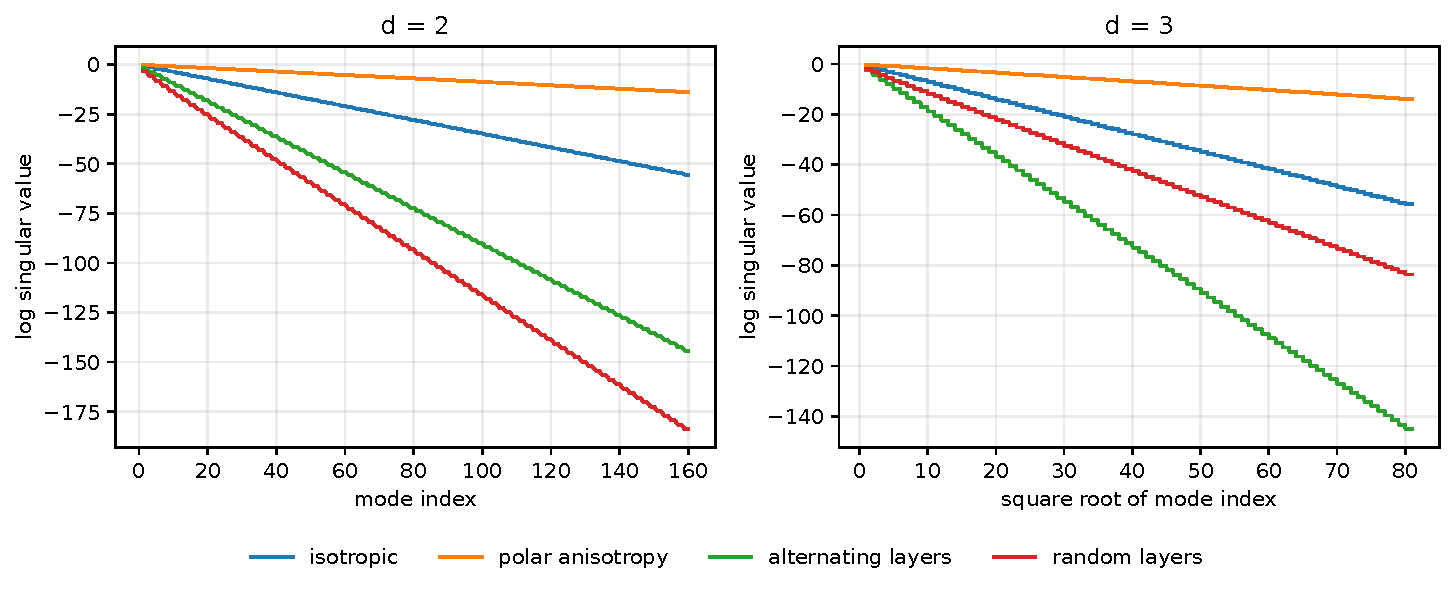
\includegraphics[width=\textwidth]{../numerical_case/figures/radial_spectra.pdf}
 \caption{Natural logarithms of finite-degree energy singular values for
 four radial cases, against $m$ or $\sqrt m$. Smaller values mean stronger
 contraction. All modes through degree $80$ are shown with multiplicity;
 no tail ordering is inferred. No values are clipped or replaced by a floor.
 These are numerical checks on a finite radial family.}\label{fig:spectra}
\end{figure}
\begin{figure}[htbp]
 \centering
 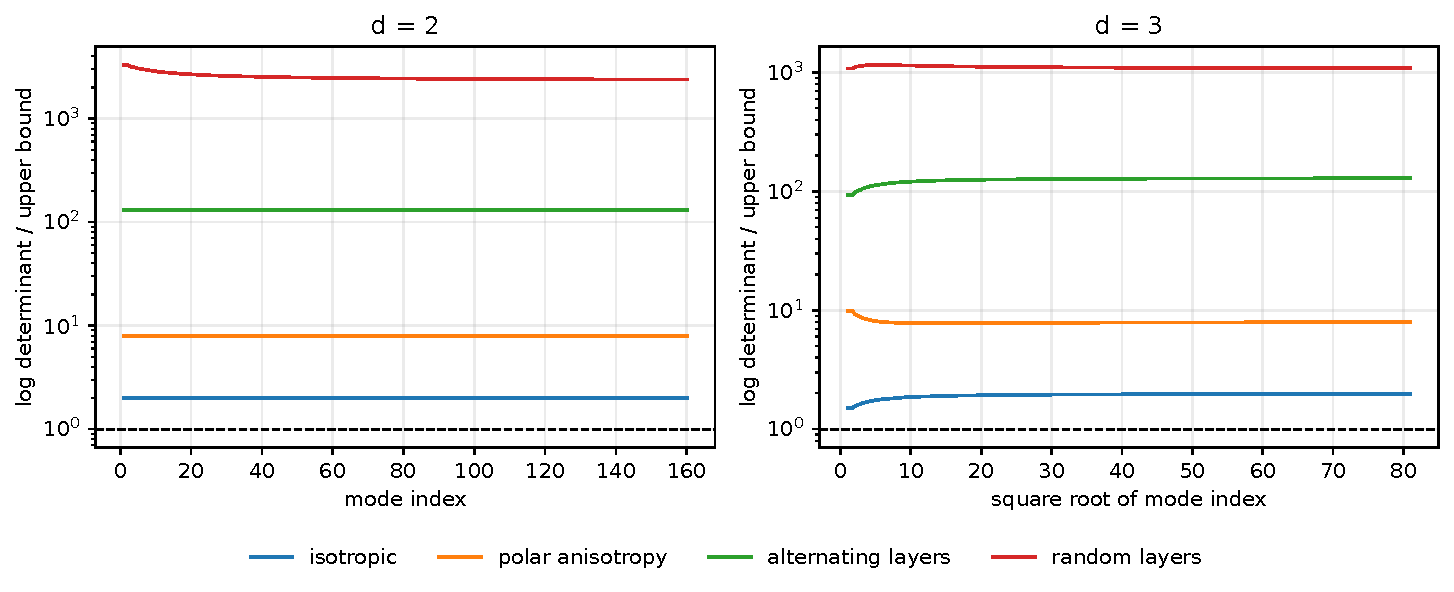
\includegraphics[width=\textwidth]{../numerical_case/figures/determinant_comparison.pdf}
 \caption{The negative-log ratio $L_m/B_m$ for the same included modes.
 Values above the dashed line at one satisfy the determinant bound.
 The vertical axis is logarithmic and the horizontal axis is $m$ or
 $\sqrt m$. Both numerator and denominator are negative; larger ratios
 indicate a stronger inequality. Every included prefix is plotted, without
 clipping or a floor.}\label{fig:det}
\end{figure}

The implementation is compared with exact constant-coefficient formulas,
independent unscaled $70$-decimal-digit matrix exponentials, and subdivision
of each annulus into two identical coefficient layers. Subdivision tests
representation invariance, rather than mesh convergence. The independent
reference constructs the matrix exponential directly and does not call
\eqref{eq:stable}. It covers both dimensions, varying contrasts and inner
radii in the core, within annuli and on interfaces.
The library has $23$ unit tests, including coefficient and geometric scaling,
invalid input rejection, spherical multiplicities and independently
derived generalized-eigenvalue examples.

There are also $40$ finite-dimensional form comparisons per dimension.
In a sphere-mode subspace of ambient dimension $40$, random orthonormal
columns form $B,Q$ using \eqref{eq:formspectrum}. A positive matrix
$G\le\beta B$ and $E'\ge\alpha Q$ are constructed with
$\alpha=0.15$, $\beta=4$. Cholesky whitening computes
$\Tr(G^{-1}E')$ and checks \eqref{eq:loggrowth}. This tests the
finite matrix inequality under its premises; it does not simulate a
general rough-coefficient PDE.

\begin{table}[htbp]
 \centering
 \caption{Recorded binary64 checks with Python 3.13.3 and NumPy 2.4.4.
 The independent reference uses mpmath at 70 decimal digits. Errors are
 absolute differences of logarithmic singular values.}\label{tab:checks}
 \begin{tabular}{lr}\toprule
 Quantity & Observed value\\\midrule
 Radial cases / finite-form trials & $40$ / $80$\\
 Largest exact constant-case error & $1.71\times10^{-13}$\\
 Largest layer-subdivision difference & $1.02\times10^{-12}$\\
 Largest determinant excess $\max(L_m-B_m)$ & $-0.30325$\\
 Smallest finite-form trace margin & $1.46480$\\\bottomrule
 \end{tabular}
\end{table}

All $40$ cases passed the determinant and individual bounds with
logarithmic tolerance $10^{-8}$; subdivision tolerance was
$2\times10^{-11}$. Exact and high-precision tolerances are specified
per test in the code. Table~\ref{tab:checks} records reproducible
numerical evidence, not interval-certified errors or a proof for all
coefficients. The prescribed layer distribution is not a statement about
typicality in the full coefficient class.

The accompanying package contains the library, unit tests, case configuration,
scripts, figures and compact summaries. Detailed arrays and an environment
manifest are regenerated locally. From its root run
\texttt{python3 -m unittest discover -s test -v} with
\texttt{PYTHONPATH=src}, then
\texttt{python3 numerical\_case/run\_cases.py} and
\texttt{python3 numerical\_case/plot\_cases.py}.
The theorem is independent of these computations.

\bibliographystyle{plain}
\bibliography{references}
\section*{AI use statement}
ChatGPT supplied an initial proof candidate and literature notes.
Codex expanded the natural-language proof, checked cited source passages,
prepared and tested the numerical implementation, and assisted with writing
and typesetting. The proof and procedures are given in full for independent
checking. These AI checks do not constitute independent human review or
formal verification.
\end{document}
